\section{Conclusion} 
In this paper, we present DisPose, a plug-and-play module for improving human image animation, which aims to provide efficient conditional control without additional dense inputs. To achieve this, we disentangle pose control into motion field guidance and keypoint correspondence. To obtain the motion field guidance, we first construct the tracking matrix from the skeleton pose, and then obtain the sparse and dense motion fields by Gaussian filtering and conditional motion diffusion, respectively. Moreover, we introduce the keypoint correspondence of diffusion features to explore the semantic correspondence in image animation. 
 Finally, we integrate the extracted guidance features into a hybrid control network. Once trained, our model can be integrated into existing human image animation models. Extensive evaluation of various models also validates the effectiveness and generalizability of our DisPose.

\begin{figure}[t]
    \centering
    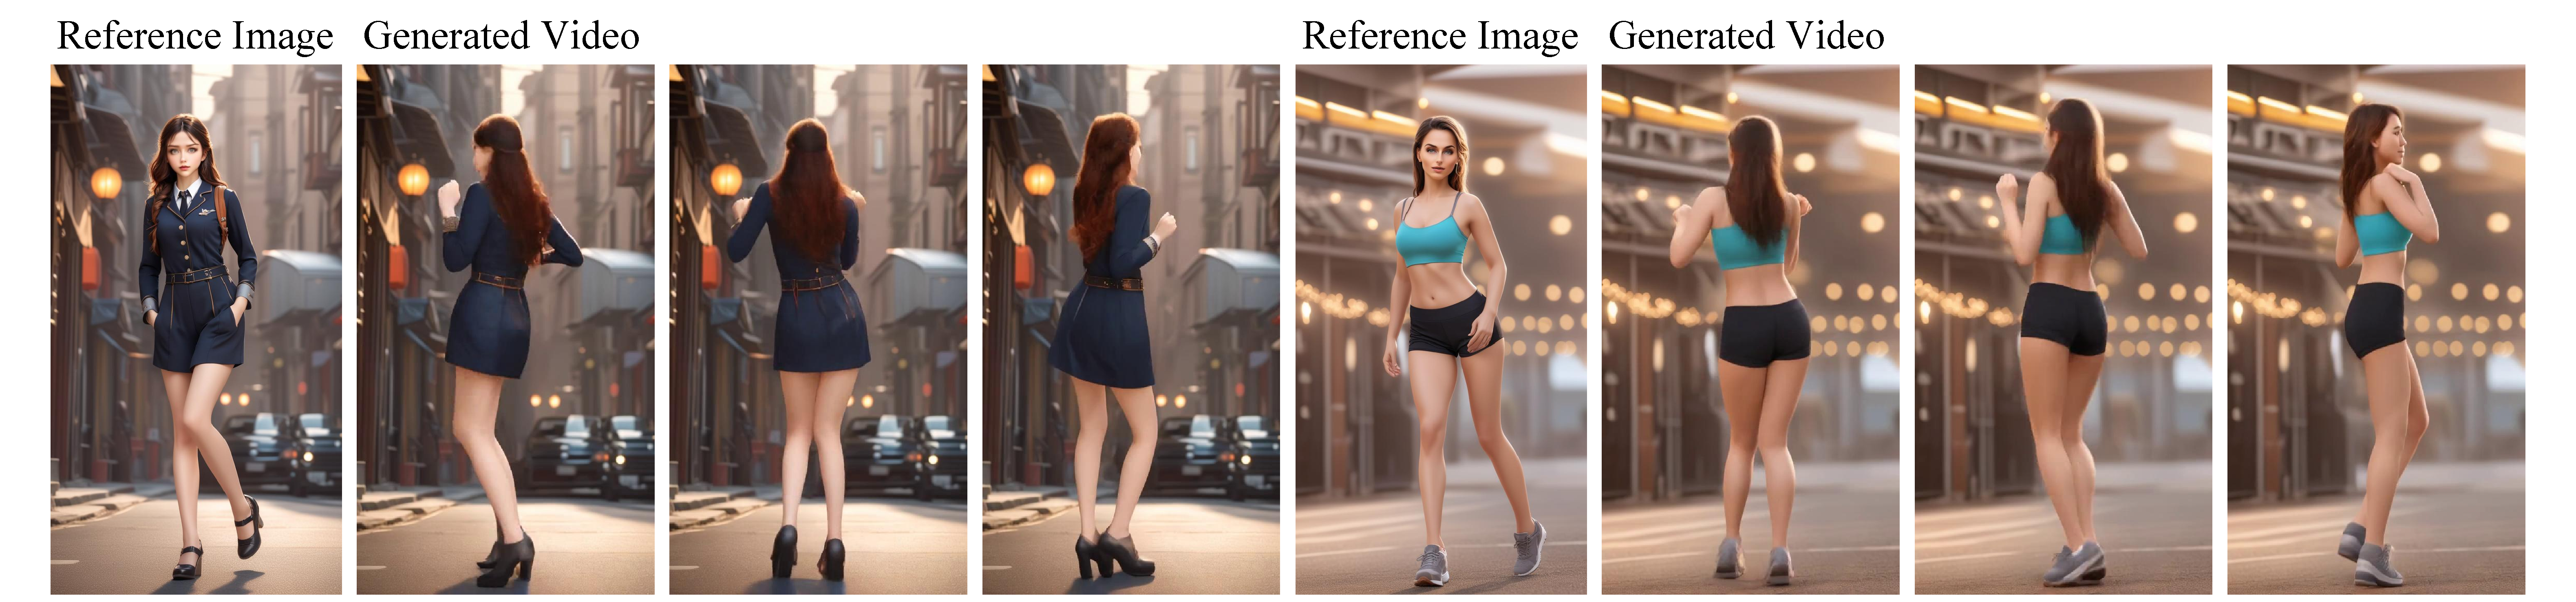
\includegraphics[width=1.0\columnwidth]{./image/limitation.pdf}
    \vspace{-15pt}
    \caption{Qualitative results of our method for multi-view video generation.}
    \label{fig: limitation}
\end{figure}

\section{Limitations and Future Works}
Despite our DisPose enhances motion guidance and appearance alignment, the ability to synthesize unseen parts for characters is still limited. As shown in Figure~\ref{fig: limitation}, we attempt to generate multi-view videos for the single-view reference image. In the future, we will explore camera control or multi-view synthesis models for capturing multi-view reference information. Moreover, introducing the 3D sparse pose as a control condition can also address this issue.
\section{Ethics Statement}
We clarify that all characters in this paper are fictional except for the TikTok~\citep{jafarian2021tiktok} dataset. We strongly condemn the misuse of generative artificial intelligence to create content that harms individuals or spreads misinformation. However, we acknowledge the potential for misuse of our approach. This is because it focuses on human-centered animation generation. We uphold the highest ethical standards in our research, including adherence to legal frameworks, respect for privacy, and encouragement to generate positive content.